
\documentclass[
	11pt, % Default font size, select one of 10pt, 11pt or 12pt
	fleqn, % Left align equations
	a4paper, % Paper size, use either 'a4paper' for A4 size or 'letterpaper' for US letter size
	%oneside, % Uncomment for oneside mode, this doesn't start new chapters and parts on odd pages (adding an empty page if required), this mode is more suitable if the book is to be read on a screen instead of printed
]{LegrandOrangeBook}
\usepackage{xeCJK}
\usepackage{fontspec}
\usepackage{ctex}
\usepackage{color}
\usepackage{caption}
\captionsetup{font={scriptsize}}
\setmainfont[]{PingFang HK}
\setCJKmainfont{Heiti SC}
% Book information for PDF metadata, remove/comment this block if not required
\hypersetup{
	pdftitle={Title}, % Title field
	pdfauthor={Author}, % Author field
	pdfsubject={Subject}, % Subject field
	pdfkeywords={Keyword1, Keyword2, ...}, % Keywords
	pdfcreator={LaTeX}, % Content creator field
}

\addbibresource{sample.bib} % Bibliography file

\definecolor{ocre}{RGB}{243, 102, 25} % Define the color used for highlighting throughout the book

\chapterimage{orange1.jpg} % Chapter heading image
\chapterspaceabove{6.5cm} % Default whitespace from the top of the page to the chapter title on chapter pages
\chapterspacebelow{6.75cm} % Default amount of vertical whitespace from the top margin to the start of the text on chapter pages


\begin{document}

\titlepage % Output the title page
{
\includegraphics[width=\paperwidth]{background.pdf}} % Code to output the background image, which should be the same dimensions as the paper to fill the page entirely; leave empty for no background image
{ % Title(s) and author(s)
	\centering\sffamily % Font styling
	{\Huge\bfseries Exploring the Physical Manifestation of Humanity's Subconscious Desires\par} % Book title
	\vspace{16pt} % Vertical whitespace
	{\LARGE A Practical Guide\par} % Subtitle
	\vspace{24pt} % Vertical whitespace
	{\huge\bfseries Goro Akechi\par} % Author name
}

%----------------------------------------------------------------------------------------
%	COPYRIGHT PAGE
%----------------------------------------------------------------------------------------

\thispagestyle{empty} % Suppress headers and footers on this page

~\vfill % Push the text down to the bottom of the page

\noindent Copyright \copyright\ 2022 Goro Akechi\\ % Copyright notice

\noindent \textsc{Published by Publisher}\\ % Publisher

\noindent \textsc{\href{https://www.latextemplates.com/template/legrand-orange-book}{book-website.com}}\\ % URL

\noindent Licensed under the Creative Commons Attribution-NonCommercial 4.0 License (the ``License''). You may not use this file except in compliance with the License. You may obtain a copy of the License at \url{https://creativecommons.org/licenses/by-nc-sa/4.0}. Unless required by applicable law or agreed to in writing, software distributed under the License is distributed on an \textsc{``as is'' basis, without warranties or conditions of any kind}, either express or implied. See the License for the specific language governing permissions and limitations under the License.\\ % License information, replace this with your own license (if any)

\noindent \textit{First printing, March 2022} % Printing/edition date

%----------------------------------------------------------------------------------------
%	TABLE OF CONTENTS
%----------------------------------------------------------------------------------------

\pagestyle{empty} % Disable headers and footers for the following pages

\tableofcontents % Output the table of contents

\listoffigures % Output the list of figures, comment or remove this command if not required

\listoftables % Output the list of tables, comment or remove this command if not required

\pagestyle{fancy} % Enable default headers and footers again

\cleardoublepage % Start the following content on a new page

%----------------------------------------------------------------------------------------
%	PART
%----------------------------------------------------------------------------------------

\part{Part One Title}

%----------------------------------------------------------------------------------------
%	SECTIONING EXAMPLES CHAPTER
%----------------------------------------------------------------------------------------

\chapterimage{orange2.jpg} % Chapter heading image
\chapterspaceabove{6.75cm} % Whitespace from the top of the page to the chapter title on chapter pages
\chapterspacebelow{7.25cm} % Amount of vertical whitespace from the top margin to the start of the text on chapter pages

%------------------------------------------------

\chapter{Pre-requisite knowledge:Basic Conception}

\section{Explanation of symbols}
在抽象代数的学习中,会使用到集合中的知识,当然也会使用到集合中的各种符号,在这一小节中,对这些符号进行一遍复习。
\subsection{不同数的符号表示}
\begin{itemize}
	\item $\mathbb{R}$ 全体实数(有理数和无理数)的集合
	\item $\mathbb{N}$ 全体自然数集合
	\item $\mathbb{N^*}$ 全体非负整数排除0的集合
	\item $\mathbb{Q}$ 全体有理数(整数和分数)的集合
	\item $\mathbb{Z}$ 全体整数的集合
	\item $\mathbb{C}$ 全体复数的集合
\end{itemize}

\subsection{集合中的常见概念符号}
\begin{itemize}
	\item 集合 A,B,C
	\item 元素 a,b,c
	\item 空集 $\emptyset$
	\item 元素与集合之间的从属关系:$\in$,$\notin$
	\item 集合与集合之间的从属关系:$\subset$,$\subseteq$,$\not\subset$
	\item 交集,补集,并集:$A\cup B$ $A\cap B$,$A^\complement$
\end{itemize}

\subsection{集合中的常见概念}
要证明两个集合相等,只需要证明这两个集合相互包含即可,这是一个非常常见的证明集合相等的手段。
\begin{theorem}
	定理一:两个集合A,B相等的充要条件:$A=B\Longleftrightarrow A\subset B\Longleftrightarrow B\subset A$
\end{theorem}
在抽象代数中,我们将使用集合的笛卡尔积来定义映射,这是一个非常重要的概念。
\begin{theorem}
	我们称:$A_1\times A_2\times ...\times A_n=\{(a_1,a_2,...,a_n)|a_i\in A_i\}$为n个集合$A_1,A_2,...A_n$的笛卡尔积。
\end{theorem}
()内表示的是有序数组,而$a_1$则表示的是$A_1$里的元素。
\begin{example}
	$$
		A=\{a,b,c\},B=\{1,2\},则
		A\times B =\{(a,1),(b,1),(c,1),(a,2),(b,2),(c,2)\}
	$$
\end{example}
根据上面这个例题,我们可以推断出一个结论。
\begin{theorem}
	一般地,如果$|A|=m,|B|=n$那么$|A\times B|=mn$
\end{theorem}
\begin{remark}
	一般,我们使用$|A|$来表示A集合中元素的个数。比如上面的$A\times B$表示的就是AB笛卡尔积所构成的集合的元素的个数。
\end{remark}

\section{mapping}
\begin{theorem}{\emph{映射的定义}}

	设$\emptyset$是从笛卡尔积$A_1\times A_2 \times ...\times A_n$到集合D的一个法则,如果$A_1\times A_2 \times ...\times A_n$中的每一个元素($a_1,a_2,...a_n$)都有D中唯一的元素d与之对应,那么我们称$\emptyset$是从$A_1\times A_2 \times ...\times A_n$到D的一个映射。
\end{theorem}
\begin{example}
	设$A_1=\{\mbox{东,西}\},A_2=\{\mbox{南}\},D=\{\mbox{高,低}\}$,
	则$\emptyset_1$(西,南)=高不是$A_1\times A_2$到D的映射,因为只定义了一种情况,总共有两种情况,没有进行一一对应。如果改为$\emptyset_2$(西,南)=高,$\emptyset_2$(东,南)=低,符合定义,所以是$A_1\times A_2$到D的映射。
\end{example}

\begin{example}
	设$A_1=D=\mathbb{R},则$

	$\emptyset(a)=a,a\not =1$\par
	$\emptyset(1)=b,b^2=1$\par
	不是$A_1$到D的映射。\par
	虽然这个映射对每一个定义域内的变量都进行了映射,但是在自变量为1的时候b可以等于+1也可以等于-1,不符合一一对应的条件,所以不是映射。
\end{example}

\begin{example}
	设$A_1=D=\mathbb{Z}_+$,则\par
	$\emptyset(a)=a-1$\par
	不是$A_1$到D的映射。\par
	由于A和D都是属于正整数集合,所以当a=1的时候映射结果不在D集合内,所以不是。
\end{example}

\begin{theorem}{映射相等}

	设$\emptyset_1,\emptyset_2$都是从笛卡尔积$A_1\times A_2 \times ...\times A_n$到集合D的映射,如果对于$A_1\times A_2 \times ...\times A_n$中的每一个元素($a_1,a_2,...,a_n$)都有
	\begin{center}
		$\emptyset_1(a_1,a_2,...,a_n)=\emptyset_2(a_1,a_2,...,a_n)$,
	\end{center}\par
	则称这两个映射$\emptyset_1,\emptyset_2$是相等的。
\end{theorem}
\begin{remark}
	特别注意:两个映射相等,实际上的要求是:
	\begin{itemize}
		\item 它们的定义域相等
		\item 它们的作用效果是相通的
	\end{itemize}
\end{remark}

\begin{example}
	设A=D都表示正整数的集合,$\emptyset_1: A\rightarrow D$ 定义为:$\emptyset_1(a)=1,\emptyset_2: A\rightarrow $定义为:$\emptyset_2(a)=a^0$,则$\emptyset_1=\emptyset_2$

	由于前提条件是正整数的集合,而不是自然数,元素自然不可能是0,所以定义域一样,而作用效果也一样,映射的结果都是1,所以映射是相等的,但是如果将本例改为自然数,则是错误的。
\end{example}
\section{algebraic operation}
\subsection{Basic Algebraic Operation}
本节的目标任务就是重新定义代数运算,打破之前对代数运算的认知,从映射与集合的观点来重新定义。

\begin{theorem}
	一个从$A\times B$到D的映射叫做一个$A\times B$到D的代数运算。
\end{theorem}


映射运算$\emptyset$:$A\times B\rightarrow D,(a,b)\rightarrow d=\emptyset(a,b)$ \par
代数运算$\circ$: $A\times B \rightarrow D,(a,b)\rightarrow d=a \circ b$

\begin{example}
	设$A=\mathbb{Z},B=\mathbb{Z}-\{0\},D=\mathbb{Q}$,则
	\begin{center}
		$\circ:(a,b)\rightarrow \frac{a}{b}=a\circ b$
	\end{center}
	是一个$A\times B$到D的代数运算,也就是普通的除法。

	\textcolor{Salmon}{对于被除数是整数,除数是不为0的整数来说,除法的运算结果既有可能是分数,也有可能是不为0的整数,所以综合来看映射自然是有理数集。}

\end{example}

\begin{example}
	设A=\{1,2\},B=\{1,2\},D=\{奇,偶\},则
	\begin{center}
		$\circ:(1,1)\rightarrow$奇,
		$(1,2)\rightarrow$奇,
		$(2,1)\rightarrow$偶,
		$(2,2)\rightarrow$偶
	\end{center}
	是一个$A\times B$到D的代数运算。

	\textcolor{Salmon}{对于$A\times$B 笛卡尔积的每一个有序数组都规定了映射的结果,并且结果都在D集合中存在,所以自然符合代数运算的含义。}
\end{example}

\begin{theorem}
	我们称$A\times A$的代数运算$\circ$为A上的代数运算,或者A上的二元运算。$\circ$具有封闭性。
\end{theorem}

\begin{example}
	设$A=\mathbb{Z}$,则普通数的加法,减法,乘法,都是集合A上的代数运算。

	\textcolor{Salmon}{结论当然是成立的,任意一个整数+整数,整数-整数,整数*整数,结果都是整数。}
\end{example}

\subsection{operational rule}
\subsubsection{associative law \&commutative law}
\begin{theorem}
	设$circ$是集合A上的一个代数运算。
	\begin{itemize}
		\item 如果对于$\forall a,b,c\in A$,都有$(a\circ b)\circ c=a\circ(b\circ c)$,则称$\circ$适合结合律。
		\item 如果对于$\forall a,b\in A$,都有$a\circ b=b\circ a$,则称$\circ$适合交换律。
	\end{itemize}
\end{theorem}

\begin{example}
	在有理数集$\mathbb{Q}$上规定代数运算$\circ$为普通加法+,那么显然$\circ$适合结合律和交换律,并且显然有:
	\begin{center}
		$[(1\circ 2)\circ(-1)]\circ(-2)=0$,

		$1\circ\{[2\circ(-1)]\circ(-2)\}=0$,

		$\{[(-2)\circ 2]\circ 1\}\circ(-1)=0$.
	\end{center}
	从这个例子可以看出,当$\circ$适合结合律和交换律的时候,\textcolor{Salmon}{任意方式加括号不改变若干个元素的乘积,任意改变元素的顺序也不改变若干元素的乘积。}
\end{example}

\begin{theorem}
	如果集合A上的代数运算适合结合律,那么任意加括号都不改变若干元素的运算结果。
\end{theorem}

\begin{theorem}
	如果集合A上的代数运算适合结合律和交换律,那么任意加括号,任意改变元素的顺序,都不改变若干元素的运算结果。
\end{theorem}

\begin{example}
	设A=\{所有不为零的实数\},$\circ$是普通数的除法$a\circ b=\frac{a}{b}$,判断$\circ$是否适合结合律。

	\textcolor{Salmon}{不适合。反例:$(36\circ 12)\circ 3=3\circ3=1$,而$36\circ (12\circ 3)=36\circ 4=9$}

\end{example}
\begin{remark}
	证明结论中,要证明一个结论是错误的,只需要举出一个反例即可。而要证明一个结论是对的,需要证明所有情况都是正确的。
\end{remark}

\begin{example}
	设A=\{a,b,c\},规定:
	\begin{center}
		\begin{table}[H]
			\centering
			\begin{tabular}{|c|c|c|c|}
				\cline{1-4}
				$\circ$ & a & b & c \\ \cline{1-4}
				a       & a & b & c \\ \cline{1-4}
				b       & b & c & a \\ \cline{1-4}
				c       & c & a & b \\ \cline{1-4}
			\end{tabular}
		\end{table}
	\end{center}
	这道题的结论是所有情况都是正确的,但是我们要证明这个结论正确,我们需要证明每一个结论都是正确的。但是如果挨个证明,总共有27个等式。我们观察a发现这是一种特殊情况,$a\circ any=any,any\circ=any$,所以a是类似于乘法中1的作用,我们根据这个特性,将情况分为x,y,z中有a和x,y,z中不存在a的情况。
	\begin{proof}
		对于任意的x,y,z$\in A$,

		1. 当x,y,z中至少有一个为a的时候,结合律成立:

		a. 当x=a的时候,$(x\circ y)\circ z=y\circ z,x\circ(y\circ z)=y\circ z$

		b. 当y=a的时候,$(x\circ y)\circ z=x\circ z,x\circ(y\circ z)=x\circ z$

		c.当z=a的时候,$(x\circ y)\circ z=x\circ y,x\circ(y\circ z)=x\circ y$

		2.当x,y,z中任何一个都不为a的时候,结合律成立,这个时候情况只有$2^3=8种$,只需要证明每一种情况均成立,则结合律成立。

		a.$(b\circ b)\circ b=c\circ b=a,b\circ(b\circ b)=b\circ c=a$

		b.$(b\circ b)\circ c=c\circ c=b,b\circ(b\circ c)=b\circ a=b$

		c.$(b\circ c)\circ b=a\circ b=b,b\circ(c\circ b)=b\circ a=b$

		d.$(b\circ c)\circ c=a\circ c=c,b\circ(c\circ c)=(b\circ b=c)$

		e.$(c\circ b)\circ b=a\circ b=b,c\circ(b\circ b)=c\circ c=b$

		f.$(c\circ b)\circ c=a\circ c=c,c\circ (b\circ c)=c\circ a=c$

		g.$(c\circ c)\circ b=b\circ b=c,c\circ (c\circ b)=c\circ a=c$

		h.$(c\circ c)\circ c=b\circ c=a,c\circ (c\circ c)=c\circ b=a$
	\end{proof}
\end{example}

\begin{example}
	设A=\{a,b,c,d\},规定:
	\begin{center}
		\begin{table}[H]
			\centering
			\begin{tabular}{|c|c|c|c|c|}
				\cline{1-5}
				$\circ$ & a & b & c                  & d                  \\ \cline{1-5}
				a       & a & b & c                  & d                  \\ \cline{1-5}
				b       & b & d & a                  & c                  \\ \cline{1-5}
				c       & c & a & b                  & \textcolor{red}{d} \\ \cline{1-5}
				d       & d & c & \textcolor{red}{a} & b                  \\ \cline{1-5}
			\end{tabular}
		\end{table}
	\end{center}
	判断$\circ$是否适合交换律。已知有限集A上的代数运算$\circ$的运算表,你能判断$\circ$是否适合交换律吗?得到的规律是什么?

	\textcolor{Salmon}{不合适,$c\circ d=d$,而$d\circ c=a$,结论:代数运算$\circ$适合交换律当且仅当其运算表中元素关于主对角线对称。}
\end{example}

\subsubsection{cancellation law}
\begin{theorem}
	设$\circ$是集合A上的一个代数运算,$\forall a,b,c\in A.$,

	1. 若$a\circ b=a\circ c\Rightarrow b=c$,则称$\circ$适合左消去律

	2. 若$b\circ a=c\circ a\Rightarrow b=c$,则称$\circ$适合右消去律。
	3. 若$\circ$既适合右消去律又适合左消去律,则称$\circ$适合消去律。
\end{theorem}

\begin{example}
	设A=\{a,b,c,d\},规定:
	\begin{center}
		\begin{table}[H]
			\centering
			\begin{tabular}{|c|c|c|c|c|}
				\cline{1-5}
				$\circ_3$ & a & b & c & d \\ \cline{1-5}
				a         & a & b & c & b \\ \cline{1-5}
				b         & b & a & d & c \\ \cline{1-5}
				c         & c & d & a & b \\ \cline{1-5}
				d         & d & c & b & a \\ \cline{1-5}
			\end{tabular}
		\end{table}
		\begin{table}[H]
			\centering
			\begin{tabular}{|c|c|c|c|c|}
				\cline{1-5}
				$\circ_4$ & a & b & c & d \\ \cline{1-5}
				a         & a & b & c & d \\ \cline{1-5}
				b         & b & a & d & c \\ \cline{1-5}
				c         & c & d & a & b \\ \cline{1-5}
				d         & d & c & b & a \\ \cline{1-5}
			\end{tabular}
		\end{table}
	\end{center}
	判断上述代数运算是否适合左消去律或右消去律。已知有限集A上的代数运算$\circ$的运算表,你能得到判断$\circ$是否适合左消去律或右消去律的规律吗?

	\textcolor{Salmon}{由于集合中元素具有互异性,每一个方格中的元素都不能相等,这也就说明如果对于一行某一个元素对应每一列的元素结果为相等的,说明不符合左消去律,而某列一个元素对应每一行的元素结果为相等的,则说明不符合右消去律。举个例子:以第一个表格中第二行a为例,对应第三列和第五列的元素都是b,$a\circ b=b,a\circ d=b\Rightarrow b=d$,由于集合元素中的互异性,$b\not=d$,所以左消去律不符合,同理右消去律也不符合。对于第二个表格,既符合左消去律,也符合右消去律,所以符合消去律。}
\end{example}

\subsection{distributive law}
特别注意,分配律是对于两种代数运算而言的,和之前的运算律不一样。
\begin{theorem}

	设$\otimes,\oplus$是集合A上的两个代数运算,$\forall a_1,a_2,b\in A$.

	1. 若$b\otimes(a_1\oplus a_2)=(b\otimes a_1)\oplus(b\otimes a_2)$,则称$\otimes$对于$\oplus$适合左分配律;

	2. 若$(a_1\oplus a_2)\otimes b=(a_1\otimes b)\oplus(a_2\otimes b)$,则称$\otimes$对于$\oplus$适合右分配律,或者第二分配律。

	3. 若$\otimes,\oplus$既适合左分配律,又适合右分配律,则称$\otimes,\oplus$适合分配律。
\end{theorem}

\section{Mapping and transformations}
\begin{theorem}
	设$\phi:A\rightarrow\bar{A}$是一个映射,对于任意的$a,b\in \bar{A}$,如果$a\not=b\Rightarrow\phi(a)\not=\phi(b)$,则称$\phi$是从A到$\bar{A}$的\emph{单射}。
\end{theorem}

\begin{theorem}
	$\phi:A\rightarrow\bar{A}$是单射当且仅当对于任意的$a,b\in\bar{A},\phi(a)=\phi(b)\Rightarrow=b$
\end{theorem}

\begin{theorem}
	设$\phi:A\rightarrow\bar{A}$是一个映射,如果对于任意的$b\in\bar{A}$,都存在$a\in A$,有$b=\phi(a)$,则称$\phi$是从A到$\bar{A}$的满射。既是单射又是满射的映射称为一一映射(双射)。
\end{theorem}

\begin{theorem}
	设$f:A\rightarrow B$和$g:B\rightarrow C$是两个映射。规定$g\circ f:A\rightarrow C$为对于任意的$x\in A$,$(g\circ f)(x)=g(f(x))$,则称$g\circ f$为f与g的复合映射。
\end{theorem}

\begin{example}
	设f(x)=sinx,g(x)=$x^3$,则f与g的复合函数为$(g\circ f)(x)=g(f(x))=sin^3x$
\end{example}

\begin{theorem}
	单射的复合是单射;满射的复合是满射;双射的复合是双射。
\end{theorem}
为了方便理解,可以来看看这几幅图进行直观对比:
\begin{figure}[H]
	\centering
	\centering
	\begin{minipage}[t]{0.25\textwidth}
		\centering
		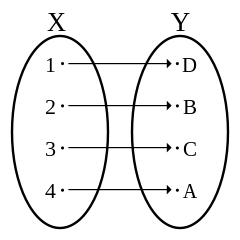
\includegraphics[width=2cm]{Images/Bijection.svg.png}
		\caption{双射}
	\end{minipage}
	\begin{minipage}[t]{0.23\textwidth}
		\centering
		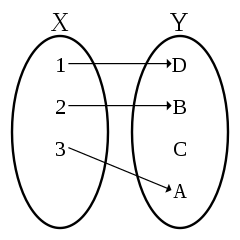
\includegraphics[width=2cm]{Images/240px-Injection.svg.png}
		\caption{单射但不满射}
	\end{minipage}
	\begin{minipage}[t]{0.23\textwidth}
		\centering
		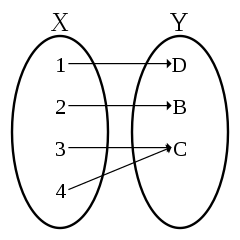
\includegraphics[width=2cm]{Images/240px-Surjection.svg.png}
		\caption{满射但不单射}
	\end{minipage}
	\begin{minipage}[t]{0.23\textwidth}
		\centering
		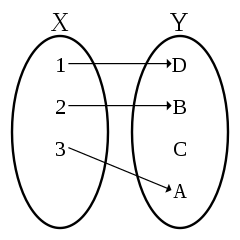
\includegraphics[width=2cm]{Images/240px-Injection.svg.png}
		\caption{单射但不满射}
	\end{minipage}
\end{figure}

\begin{vocabulary}[单射]
	指将不同的变量映射到不同的值的函数
\end{vocabulary}

\begin{vocabulary}[满射]
	指陪域等于值域的函数。
\end{vocabulary}
\begin{vocabulary}[双射]
	既是单射又是满射的函数
\end{vocabulary}

\begin{theorem}
	设$f:A\rightarrow B$和$g:B\rightarrow A$是两个映射。如果$f\circ g=id_B:B\rightarrow B$且$g\circ f=id_A:A\Rightarrow A$,则称f与g互为逆映射。
\end{theorem}


\begin{theorem}
	双射存在唯一的逆映射,且这个逆映射也是双射
\end{theorem}

\begin{proof}
	设$f:A\rightarrow B$是一个双射.

	\textcolor{Salmon}{我们规定$f^{-1}:B\rightarrow A$ 为对于任意的$y=f(x)\in B,f^{-1}(y)=x$,即原像运算。由于f是满射,说明B集合中的每一个元素都可以对应A中唯一的元素,这符合映射的定义(详情可以看笛卡尔积定义映射的部分),所以通过满射的条件,我们证明了双射存在逆映射}

	\textcolor{teal}{接下来我们应该证明逆映射是一个单射。任意取$f(x_1)=y_1\not=y_2=f(x_2)\in B$,这个是根据f是单射可以得到的,所以$f^{-1}(y_1)=x_1\not=x_2=f^{-1}(y_2)$,根据$x_1\not=x_2$作为媒介,我们推出了$f^{-1}(y_1)\not=f^{-1}(y_2)$,从而可以证明$f^{-1}$是单射}

	\textcolor{blue}{接下来证明逆映射是满射的情况,这个的证明和证明单射是非常像的,由于f是映射,任取$x\in A$,$f(x)=y\in B$。这说明了x在$f^{-1}$的原像是存在的,从而$f^{-1}$自然是满射}。

	\textcolor{black}{然后需要证明$f^{-1}$是f的逆映射。对于任意的$x\in A,$如果令$x_1=(f^{-1}\circ f)(x)$,则$x_1=f^{-1}(f(x))$,从而$f(x)=f(x_1)$。由于f是单射,所以可以得到$x_1=x$,于是x=$(f^{-1}\circ f)(x)$对于任意的$x\in A$都成立。这就证明了$f^{-1}\circ f=id_A$,同理可证$f\circ f^{-1}=id_B$}

	\textcolor{gray}{最后需要证明逆映射的唯一性,设g也是f的一个逆映射,则由于逆映射的定义必然有$g\circ f=id_A,f\circ g=id_B$,所以$g=g\circ id_B=g\circ(f\circ f^{-1}=(g\circ f)\circ f^{-1})=id_A\circ f^{-1}=f^{-1}$}
\end{proof}

\begin{definition}
	一个A到A得映射叫做A的一个变换。一个A到A的单射,满射,或A与A之间的一一映射(双射)叫做A的一个单射变换,满射变换或一一变换。
\end{definition}

\begin{theorem}
	变换的复合适合结合律。
\end{theorem}

\begin{proof}
	设T表示集合A上所有的变换的集合,对于任意的$f,g,h\in T,$因为对于任意的$x\in A,$:

	$((f\circ g)\circ h)(x)=(f\circ g)(h(x))=f(g(h(x)))$,

	$(f\circ(g\circ h))(x)=f((g\circ h)(x))=f(g(h(x)))$

	最后根据映射相等的定义,立即推$(f\circ g)\circ h=f(\circ(g\circ h))$
\end{proof}

\begin{example}
	假定$\phi$是A与$\bar{A}$之间的一一映射,$a\in A$,则$\phi^{-1}[\phi(a)]=? \phi[\phi^{-1}(a)]=?$

	若$phi$是A的一一变换,这两个问题的结果又是什么?

	\textcolor{Salmon}{
		\begin{enumerate}
			\item $\phi$是A与$\bar{A}$之间的一一映射,$\phi^{-1}[\phi(a)]=a,\phi[\phi^{-1}(a)]$一般不存在,因为一一映射是从A$\Rightarrow B$的一个映射,在B中不一定定义域包括$\phi(a)$
			\item $\phi$是A的一个一一变换的时候,两式都等于a,对于第二条可以使用变换的结合律来得到结果$\phi^[\phi^{-1}(a)]=\phi^{-1}[\phi(a)]=a$,关键在于此时$\phi(a),a$都在A中,一定有定义。
		\end{enumerate}
	}
\end{example}
\chapter{In-text Element Examples}



%------------------------------------------------

\section{Lists}\index{Lists}

Lists are useful to present information in a concise and/or ordered way.

\subsection{Numbered List}\index{Lists!Numbered List}

\begin{enumerate}
	\item First numbered item
	      \begin{enumerate}
		      \item First indented numbered item
		      \item Second indented numbered item
		            \begin{enumerate}
			            \item First second-level indented numbered item
		            \end{enumerate}
	      \end{enumerate}
	\item Second numbered item
	\item Third numbered item
\end{enumerate}

\subsection{Bullet Point List}\index{Lists!Bullet Points}

\begin{itemize}
	\item First bullet point item
	      \begin{itemize}
		      \item First indented bullet point item
		      \item Second indented bullet point item
		            \begin{itemize}
			            \item First second-level indented bullet point item
		            \end{itemize}
	      \end{itemize}
	\item Second bullet point item
	\item Third bullet point item
\end{itemize}

\subsection{Descriptions and Definitions}\index{Lists!Descriptions and Definitions}

\begin{description}
	\item[Name] Description
	\item[Word] Definition
	\item[Comment] Elaboration
\end{description}

%------------------------------------------------

\section{International Support}

àáâäãåèéêëìíîïòóôöõøùúûüÿýñçčšž

\noindent ÀÁÂÄÃÅÈÉÊËÌÍÎÏÒÓÔÖÕØÙÚÛÜŸÝÑ

\noindent ßÇŒÆČŠŽ

%------------------------------------------------

\section{Ligatures}

fi fj fl ffl ffi Ty

%----------------------------------------------------------------------------------------
%	PART
%----------------------------------------------------------------------------------------

\part{Part Two Title}

%----------------------------------------------------------------------------------------
%	MATHEMATICS EXAMPLES CHAPTER
%----------------------------------------------------------------------------------------

\chapter{Mathematics}

\section{Theorems}\index{Theorems}

\subsection{Several equations}\index{Theorems!Several Equations}

This is a theorem consisting of several equations.

\begin{theorem}[Name of the theorem] % Specify a name/title in square brackets, or leave them out for no title
	In $E=\mathbb{R}^n$ all norms are equivalent. It has the properties:
	\begin{align}
		 & \big| ||\mathbf{x}|| - ||\mathbf{y}|| \big|\leq || \mathbf{x}- \mathbf{y}||                            \\
		 & ||\sum_{i=1}^n\mathbf{x}_i||\leq \sum_{i=1}^n||\mathbf{x}_i||\quad\text{where $n$ is a finite integer}
	\end{align}
\end{theorem}

\subsection{Single Line}\index{Theorems!Single Line}

This is a theorem consisting of just one line.

\begin{theorem} % Specify a name/title in square brackets, or leave them out for no title
	A set $\mathcal{D}(G)$ in dense in $L^2(G)$, $|\cdot|_0$.
\end{theorem}

%------------------------------------------------

\section{Definitions}\index{Definitions}

A definition can be mathematical or it could define a concept.

\begin{definition}[Definition name] % Specify a name/title in square brackets, or leave them out for no title
	Given a vector space $E$, a norm on $E$ is an application, denoted $||\cdot||$, $E$ in $\mathbb{R}^+=[0,+\infty[$ such that:
	\begin{align}
		 & ||\mathbf{x}||=0\ \Rightarrow\ \mathbf{x}=\mathbf{0}        \\
		 & ||\lambda \mathbf{x}||=|\lambda|\cdot ||\mathbf{x}||        \\
		 & ||\mathbf{x}+\mathbf{y}||\leq ||\mathbf{x}||+||\mathbf{y}||
	\end{align}
\end{definition}

%------------------------------------------------

\section{Notations}\index{Notations}

\begin{notation} % Specify a name/title in square brackets, or leave them out for no title
	Given an open subset $G$ of $\mathbb{R}^n$, the set of functions $\varphi$ are:
	\begin{enumerate}
		\item Bounded support $G$;
		\item Infinitely differentiable;
	\end{enumerate}
	a vector space is denoted by $\mathcal{D}(G)$.
\end{notation}

%------------------------------------------------

\section{Remarks}\index{Remarks}

This is an example of a remark.

\begin{remark}
	The concepts presented here are now in conventional employment in mathematics. Vector spaces are taken over the field $\mathbb{K}=\mathbb{R}$, however, established properties are easily extended to $\mathbb{K}=\mathbb{C}$.
\end{remark}

%------------------------------------------------

\section{Corollaries}\index{Corollaries}

\begin{corollary}[Corollary name] % Specify a name/title in square brackets, or leave them out for no title
	The concepts presented here are now in conventional employment in mathematics. Vector spaces are taken over the field $\mathbb{K}=\mathbb{R}$, however, established properties are easily extended to $\mathbb{K}=\mathbb{C}$.
\end{corollary}

%------------------------------------------------

\section{Propositions}\index{Propositions}

\subsection{Several equations}\index{Propositions!Several Equations}

\begin{proposition}[Proposition name] % Specify a name/title in square brackets, or leave them out for no title
	It has the properties:
	\begin{align}
		 & \big| ||\mathbf{x}|| - ||\mathbf{y}|| \big|\leq || \mathbf{x}- \mathbf{y}||                            \\
		 & ||\sum_{i=1}^n\mathbf{x}_i||\leq \sum_{i=1}^n||\mathbf{x}_i||\quad\text{where $n$ is a finite integer}
	\end{align}
\end{proposition}

\subsection{Single Line}\index{Propositions!Single Line}

\begin{proposition} % Specify a name/title in square brackets, or leave them out for no title
	Let $f,g\in L^2(G)$; if $\forall \varphi\in\mathcal{D}(G)$, $(f,\varphi)_0=(g,\varphi)_0$ then $f = g$.
\end{proposition}

%------------------------------------------------

\section{Examples}\index{Examples}

\subsection{Equation Example}\index{Examples!Equation}

\begin{example} % Specify a name/title in square brackets, or leave them out for no title
	Let $G=\{x\in\mathbb{R}^2:|x|<3\}$ and denoted by: $x^0=(1,1)$; consider the function:
	\begin{equation}
		f(x)=\left\{\begin{aligned}                                                                                                                                                                                                                                                                                                                                                                                 & \mathrm{e}^{|x|} &  & \text{si $|x-x^0|\leq 1/2$} \\
                                                                                                                                                                                                                                                                                                                                                                                                & 0                &  & \text{si $|x-x^0|> 1/2$}\end{aligned}\right.
	\end{equation}
	The function $f$ has bounded support, we can take $A=\{x\in\mathbb{R}^2:|x-x^0|\leq 1/2+\epsilon\}$ for all $\epsilon\in\mathopen{]}0\,;5/2-\sqrt{2}\mathclose{[}$.
\end{example}

\subsection{Text Example}\index{Examples!Text}

\begin{example}[Example name] % Specify a name/title in square brackets, or leave them out for no title
	Aliquam arcu turpis, ultrices sed luctus ac, vehicula id metus. Morbi eu feugiat velit, et tempus augue. Proin ac mattis tortor. Donec tincidunt, ante rhoncus luctus semper, arcu lorem lobortis justo, nec convallis ante quam quis lectus. Aenean tincidunt sodales massa, et hendrerit tellus mattis ac. Sed non pretium nibh. Donec cursus maximus luctus. Vivamus lobortis eros et massa porta porttitor.
\end{example}

%------------------------------------------------

\section{Exercises}\index{Exercises}

\begin{exercise} % Specify a name/title in square brackets, or leave them out for no title
	This is a good place to ask a question to test learning progress or further cement ideas into students' minds.
\end{exercise}

%------------------------------------------------

\section{Problems}\index{Problems}

\begin{problem} % Specify a name/title in square brackets, or leave them out for no title
What is the average airspeed velocity of an unladen swallow?
\end{problem}

%------------------------------------------------

\section{Vocabulary}\index{Vocabulary}

Define a word to improve a students' vocabulary.

\begin{vocabulary}[Word] % Specify a name/title in square brackets, or leave them out for no title
	Definition of word.
\end{vocabulary}

%----------------------------------------------------------------------------------------
%	PRESENTING INFORMATION/RESULTS EXAMPLES CHAPTER
%----------------------------------------------------------------------------------------

\chapterimage{orange3.jpg} % Chapter heading image
\chapterspaceabove{6.25cm} % Whitespace from the top of the page to the chapter title on chapter pages
\chapterspacebelow{7.5cm} % Amount of vertical whitespace from the top margin to the start of the text on chapter pages

%------------------------------------------------

\chapter{Presenting Information and Results with a Long Chapter Title}

\section{Table}\index{Table}

Lorem ipsum dolor sit amet, consectetur adipiscing elit. Praesent porttitor arcu luctus, imperdiet urna iaculis, mattis eros. Pellentesque iaculis odio vel nisl ullamcorper, nec faucibus ipsum molestie. Sed dictum nisl non aliquet porttitor. Etiam vulputate arcu dignissim, finibus sem et, viverra nisl. Aenean luctus congue massa, ut laoreet metus ornare in. Nunc fermentum nisi imperdiet lectus tincidunt vestibulum at ac elit. Nulla mattis nisl eu malesuada suscipit.

\begin{table}[H] % Use [H] to suppress floating and place the figure/table exactly where it is specified in the text
	\centering % Horizontally center the table on the page
	\begin{tabular}{L{0.15\textwidth} R{0.15\textwidth} R{0.15\textwidth}} % Specify column alignment with L{width}, C{width} and R{width} for fixed-width columns, or the default latex l, c and r for flexible-width columns
		\toprule
		\textbf{Treatments} & \textbf{Response 1} & \textbf{Response 2} \\
		\midrule
		Treatment 1         & 0.0003262           & 0.562               \\
		Treatment 2         & 0.0015681           & 0.910               \\
		Treatment 3         & 0.0009271           & 0.296               \\
		\bottomrule
	\end{tabular}
	\caption{Table caption.}
	\label{tab:example} % Unique label used for referencing the table in-text
\end{table}

Referencing \autoref{tab:example} in-text using its label.

\begin{table}[t] % Floating table, [t] tells LaTeX to place it at the top of the next available page
	\centering % Horizontally center the table on the page
	\begin{tabular}{L{0.15\textwidth} R{0.15\textwidth} R{0.15\textwidth}} % Specify column alignment with L{width}, C{width} and R{width} for fixed-width columns, or the default latex l, c and r for flexible-width columns
		\toprule
		\textbf{Treatments} & \textbf{Response 1} & \textbf{Response 2} \\
		\midrule
		Treatment 1         & 0.0003262           & 0.562               \\
		Treatment 2         & 0.0015681           & 0.910               \\
		Treatment 3         & 0.0009271           & 0.296               \\
		\bottomrule
	\end{tabular}
	\caption{Floating table.}
	\label{tab:floating} % Unique label used for referencing the table in-text
\end{table}

%------------------------------------------------

\section{Figure}\index{Figure}

Lorem ipsum dolor sit amet, consectetur adipiscing elit. Praesent porttitor arcu luctus, imperdiet urna iaculis, mattis eros. Pellentesque iaculis odio vel nisl ullamcorper, nec faucibus ipsum molestie. Sed dictum nisl non aliquet porttitor. Etiam vulputate arcu dignissim, finibus sem et, viverra nisl. Aenean luctus congue massa, ut laoreet metus ornare in. Nunc fermentum nisi imperdiet lectus tincidunt vestibulum at ac elit. Nulla mattis nisl eu malesuada suscipit.

\begin{figure}[H] % Use [H] to suppress floating and place the figure/table exactly where it is specified in the text
	\centering % Horizontally center the figure on the page
	
\includegraphics[width=0.5\textwidth]{creodocs_logo.pdf} % Include the figure image
	\caption{Figure caption.}
	\label{fig:placeholder} % Unique label used for referencing the figure in-text
\end{figure}

Referencing \autoref{fig:placeholder} in-text using its label.

\begin{figure}[b] % Floating figure, [b] tells LaTeX to place it at the bottom of the next available page
	\centering % Horizontally center the figure on the page
	
\includegraphics[width=\textwidth]{creodocs_logo.pdf} % Include the figure image
	\caption{Floating figure.}
	\label{fig:floating} % Unique label used for referencing the figure in-text
\end{figure}

%----------------------------------------------------------------------------------------

\stopcontents[part] % Manually stop the 'part' table of contents here so the previous Part page table of contents doesn't list the following chapters

%----------------------------------------------------------------------------------------
%	BIBLIOGRAPHY
%----------------------------------------------------------------------------------------

\chapterimage{} % Chapter heading image
\chapterspaceabove{2.5cm} % Whitespace from the top of the page to the chapter title on chapter pages
\chapterspacebelow{2cm} % Amount of vertical whitespace from the top margin to the start of the text on chapter pages

%------------------------------------------------

\chapter*{Bibliography}
\markboth{\sffamily\normalsize\bfseries Bibliography}{\sffamily\normalsize\bfseries Bibliography} % Set the page headers to display a Bibliography chapter name
\addcontentsline{toc}{chapter}{\textcolor{ocre}{Bibliography}} % Add a Bibliography heading to the table of contents

\section*{Articles}
\addcontentsline{toc}{section}{Articles} % Add the Articles subheading to the table of contents

\printbibliography[heading=bibempty, type=article] % Output article bibliography entries

\section*{Books}
\addcontentsline{toc}{section}{Books} % Add the Books subheading to the table of contents

\printbibliography[heading=bibempty, type=book] % Output book bibliography entries

%----------------------------------------------------------------------------------------
%	INDEX
%----------------------------------------------------------------------------------------

\cleardoublepage % Make sure the index starts on an odd (right side) page
\phantomsection
\addcontentsline{toc}{chapter}{\textcolor{ocre}{Index}} % Add an Index heading to the table of contents
\printindex % Output the index

%----------------------------------------------------------------------------------------
%	APPENDICES
%----------------------------------------------------------------------------------------

\chapterimage{orange2.jpg} % Chapter heading image
\chapterspaceabove{6.75cm} % Whitespace from the top of the page to the chapter title on chapter pages
\chapterspacebelow{7.25cm} % Amount of vertical whitespace from the top margin to the start of the text on chapter pages

\begin{appendices}

	\renewcommand{\chaptername}{Appendix} % Change the chapter name to Appendix, i.e. "Appendix A: Title", instead of "Chapter A: Title" in the headers

	%------------------------------------------------

	\chapter{Appendix Chapter Title}

	\section{Appendix Section Title}

	Lorem ipsum dolor sit amet, consectetur adipiscing elit. Aliquam auctor mi risus, quis tempor libero hendrerit at. Duis hendrerit placerat quam et semper. Nam ultricies metus vehicula arcu viverra, vel ullamcorper justo elementum. Pellentesque vel mi ac lectus cursus posuere et nec ex. Fusce quis mauris egestas lacus commodo venenatis. Ut at arcu lectus. Donec et urna nunc. Morbi eu nisl cursus sapien eleifend tincidunt quis quis est. Donec ut orci ex. Praesent ligula enim, ullamcorper non lorem a, ultrices volutpat dolor. Nullam at imperdiet urna. Pellentesque nec velit eget est euismod pretium.

	%------------------------------------------------

	\chapter{Appendix Chapter Title}

	\section{Appendix Section Title}

	Lorem ipsum dolor sit amet, consectetur adipiscing elit. Aliquam auctor mi risus, quis tempor libero hendrerit at. Duis hendrerit placerat quam et semper. Nam ultricies metus vehicula arcu viverra, vel ullamcorper justo elementum. Pellentesque vel mi ac lectus cursus posuere et nec ex. Fusce quis mauris egestas lacus commodo venenatis. Ut at arcu lectus. Donec et urna nunc. Morbi eu nisl cursus sapien eleifend tincidunt quis quis est. Donec ut orci ex. Praesent ligula enim, ullamcorper non lorem a, ultrices volutpat dolor. Nullam at imperdiet urna. Pellentesque nec velit eget est euismod pretium.

	%------------------------------------------------

\end{appendices}

%----------------------------------------------------------------------------------------

\end{document}
